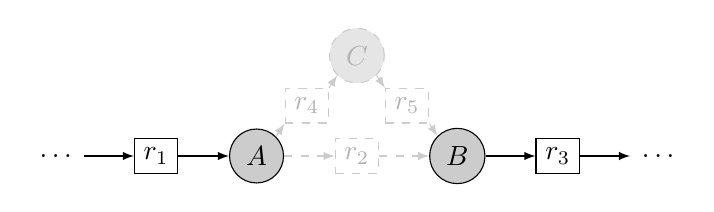
\begin{tikzpicture}[scale=0.85]
  \tikzstyle{metabolite}=[draw,circle,fill=white!80!black];
  \tikzstyle{dots}=[draw,white,circle,text=black];
  \tikzstyle{repairmetabolite}=[draw,white!80!black, circle,fill=white!90!black,text=white!70!black,dashed];
  \tikzstyle{seed}=[draw,circle,fill=BlueGreen!70];%white!80!black
  \tikzstyle{target}=[draw,circle,fill=YellowOrange];%white!40!black
  \tikzstyle{reaction}=[draw,rectangle];
  \tikzstyle{repairreaction}=[draw,rectangle,white!80!black,text=white!70!black,dashed];
  \tikzstyle{initial}=[->,>=latex,thick];
  \tikzstyle{bdd}=[->,>=latex,thick];
  \tikzstyle{etiq}=[midway,fill=black!20,scale=0.5];
  
  
  \node[dots] (in) at (1,6.5) {$\dots$};
  \node[dots] (out) at (10,6.5) {$\dots$};
  \node[metabolite] (A) at (4,6.5) {$A$};
  \node[metabolite] (B) at (7,6.5) {$B$};
  \node[repairmetabolite] (C) at (5.5,8) {$C$};
  
  \node[reaction] (R1) at (2.5,6.5) {$r_{1}$};
  \node[repairreaction] (R2) at (5.5,6.5) {$r_{2}$};
  \node[reaction] (R3) at (8.5,6.5) {$r_{3}$};
  \node[repairreaction] (R4) at (4.75,7.25) {$r_{4}$};
  \node[repairreaction] (R5) at (6.25,7.25) {$r_{5}$};
    
  % R1 : in => A
  \draw[->,>=latex] (in.east) -- (R1.west);
  \draw[->,>=latex] (R1.east) -- (A.west);
  
  % R2 : A => B
  \draw[->,>=latex,white!80!black,dashed] (A.east) -- (R2.west);
  \draw[->,>=latex,white!80!black,dashed] (R2.east) -- (B.west);
  
  % R3 : B => out
  \draw[->,>=latex] (B.east) -- (R3.west);
  \draw[->,>=latex] (R3.east) -- (out.west);
  
  % R4 : A => C
  \draw[->,>=latex,white!80!black,dashed] (A.north east) -- (R4.south west);
  \draw[->,>=latex,white!80!black,dashed] (R4.north east) -- (C.south west);
  
  % R5 : C => B
  \draw[->,>=latex,white!80!black,dashed] (C.south east) -- (R5.north west);
  \draw[->,>=latex,white!80!black,dashed] (R5.south east) -- (B.north west);
  
\end{tikzpicture}
%
%%% Local Variables:
%%% mode: latex
%%% TeX-master: "paper"
%%% End:
